%%%%%%%%%%%%%%%%%%%%%%%%%%%%%%%%%%%%%%%%%%%%%%%%%%%%%%%%%%%%%%%%%%%%%%%%
%                                                                      %
% LaTeX, FIIW thesis template                                          %
% 28/11/2014 v1.2                                                      %
%                                                                      %
%%%%%%%%%%%%%%%%%%%%%%%%%%%%%%%%%%%%%%%%%%%%%%%%%%%%%%%%%%%%%%%%%%%%%%%%
\documentclass[11pt,a4paper]{report}
% Indien je je thesis recto-verso wil afdrukken gebruik je onderstaande opties i.p.v. bovenstaande
%\documentclass[11pt,a4paper,twoside,openright]{report}

\usepackage[a4paper,left=3.5cm, right=2.5cm, top=3.5cm, bottom=3.5cm]{geometry}
\usepackage[dutch]{babel}
\usepackage{graphicx}
\usepackage[latin1]{inputenc}           % om niet ascii karakters rechtstreeks te kunnen inputten
%\usepackage[utf8]{inputenc}            % commentarieer deze regel uit als je utf8 encoded files gebruikt in plaats van latin1
\usepackage{natbib}
\usepackage{listings}             		% voor het weergeven van broncode
\usepackage{verbatim}					% weergeven van code, commando's, ...
\usepackage{hyperref}					% maak PDF van de thesis navigeerbaar
\usepackage{url}						% URL's invoegen in tekst met behulp van \url{http://}
\usepackage[small,bf,hang]{caption}     % om de captions wat te verbeteren
\usepackage[final]{pdfpages}            % gebruikt voor het invoegen van het artikel in pdf-formaat
\usepackage{pslatex}					% andere lettertype's dan de standaard types

\usepackage{sectsty}					% aanpassen van de fonts van sections en chapters
\allsectionsfont{\sffamily}
\chapterfont{\raggedleft\sffamily}

\usepackage{float}                      % De optie H voor de plaatsing van figuren op de plaats waar je ze invoegt. bvb. \begin{figure}[H]
%\usepackage{longtable}					% tabellen die over meerdere pagina's gespreid worden
%\usepackage[times]{quotchap}           % indien je fancy hoofdstuktitels wil
%\usepackage[none]{hyphenat}
%\usepackage{latexsym}
%\usepackage{amsmath}
%\usepackage{amssymb}

\usepackage{fiiw_denayer}
% \usepackage{fiiw_denayer_eng} % For the english version (also change last page at the bottom of this file!

%door onderstaande regels in commentaar te zetten, of op false, kan je pagina's weglaten
%bijvoorbeeld het weglaten van een voorwoord, lijst met symbolen, ...
%%%%%%%%%%%%%%%%%%%%%%%%%%%%%%%%%%%%%%%%%%%%%%%%%%%%%%%%%%%%%%%%%%%%%%%%%%%%%%%%%%%%%%%%
%voorwoord toevoegen?
\acknowledgementspagetrue
\acknowledgements{voorwoord}			%.tex file met daarin het voorwoord
%abstract toevoegen?
\abstractpagetrue
\abstracts{abstract}					%.tex file met daarin het abstract
%lijst van figuren toevoegen?
\listoffigurespagetrue
%lijst van tabellen toevoegen?
\listoftablespagetrue
%lijst van symbolen toevoegen?
\listofsymbolspagetrue
\listofsymbols{symbolen}				%.tex file met daarin de lijst van symbolen



%informatie over het eindwerk, de promotor, ...
%%%%%%%%%%%%%%%%%%%%%%%%%%%%%%%%%%%%%%%%%%%%%%%
\opleiding{Elektronica -ICT}
\afdeling{ICT}

\title{Geoptimaliseerde surveillance van een broadcaster voor real-time distribute van GNSS data stromen}
\subtitle{ }
% \author{naam student}
\forename{Nele}
\surname{Annaert}
\academicyear{2017 - 2018}

\promotorA[Promotor(en)]{Mevr. Ann Philips}
\promotorB[Co-promotor(en)]{Dr. Carine Bruyninx\\(My company promotor)}

\begin{document}
\selectlanguage{dutch}
% \selectlanguage{english} % For the english version
\preface

 %
\newcommand*{\MyIndentSit}{\hspace*{1 cm}}%

\chapter{Situering en doelstelling}
\label{Situering}
Het onderwerp van deze masterproef is: \newline
\MyIndentSit Geoptimaliseerde surveillance van een broadcaster voor real-time distribute van GNSS data stromen


Dit wordt onwikkeld samen met de Koninklijke Sterrenwacht van Belgi\"e. Voor het verder verloop van de masterproef, wordt hiernaar verwezen als de Royal Observatory of Belgium (ROB). Figuur \ref{imgROB} toont het logo van het ROB. De verdere uitleg over de situering van de masterproef staat in sectie \ref{SSit}.

\begin{figure}[hpb]
	
\includegraphics[scale=1]{ROB.jpg}
	\caption{Logo van de Koninklijke Sterrenwacht van Belgi\"e \cite{SImgROB}}
	\label{imgROB}
\end{figure} 

Het doel om het gebruik van data afkomstig van satellieten te bestuderen. Het doel wordt verder in detail besproken in sectie \ref{SDoe}.

\section{Situering}
\label{SSit}
Er zijn verschillende constellaties die deel uitmaken van het GNSS. In sectie \ref{LGNS} worden deze verder in detail besproken. Deze constellaties zijn opbebouwd uit satellieten. De data van deze satellieten wordt verzameld door het EUREF Permanent Network (EPN), hierover is meer informatie te vinden in sectie \ref{LEPN}. Het ROB doet dienst als het centrale bureau van het EPN. Hierdoor zijn zij verantwoordelijk voor het beheer van de data. In deze masterproef wordt verder ingegaan op het beheer van deze data en de logfiles. Deze worden verzameld door de broadcaster die gebruikt wordt om de data verder te verspreiden naar bevoegde instanties. Voorafgaand was er nog geen onderzoek gebeurd naar de logfiles van de broadcaster. Na de masterproef zou het voor de medewerkers van het ROB duidelijk moeten zijn wat er in de logfile staat. Dit moet grafisch weergegeven worden. Eveneens zou voor de verantwoordelijke het dagelijks beheer hierdoor eenvoudiger moeten worden. 

\section{Doel}
\label{SDoe}
Deze masterproef heeft volgende onderzoeksvraag: \newline
\MyIndentSit Welke gegevens worden door het logging systeem van de GNSS broadcaster verzameld? \newline
\MyIndentSit Is het mogelijk om met deze gegevens het beheer van de GNSS broadcaster te vergemakkelijken?\newline
\MyIndentSit Welke aanpassingen moeten in de software gebeurden zodat de doelstellingen verwezenlijkt kunnen worden? 
In de literatuurstudie (in hoofdstuk \ref{Literatuurstudie}) wordt in de eerste plaats gekeken naar de nodige kennis over satellieten, GNSS en de communicatie, om het practisch gedeelte van de masterproef te kunnen begrijpen.
\newline
Deze masterproef heeft als uiteindelijk doel een nieuw geoptimaliseerd logging systeem voor de GNSS broadcaster te ontwerpen. Deze broeadcaster moet uiteindelijk in staat zijn om:
\begin{itemize}
	\item Detecteren en reageren op potenti\"ele beveiligings problemen. (Zoals bijvoorbeeld herhaaldelijk proberen aanmelden met een verkeerd paswoord, veel simultane verbindingen ...)
	\item Feedback geven aan de leveranciers van datastromen over het gebruik van hun data
	\item Bestuderen van de status/gezondheid van clients, sofware gebruikt voor het maken van de verbinding, het gebruikt protocol, verbruik van de bandbreedte ...
\end{itemize}
Het zou kunnen dat om dit te verwezelijken de software van de logger aangepast moet worden zodat er meer data bewaart wordt. De verkregen informatie moet grafisch worden voorgesteld op een web-gebaseerde interface.  Deze interface moet voor de verantwoordelijke van de configuratie van de broadcaster het dagelijks beheer vergemakkelijken. 
%Het eerste hoofdstuk van je thesis.
\chapter{Literatuurstudie}
De literatuurstudie schetst een beeld van de sateliet constellaties die gebruikt worden. Deze worden besproken in \ref{LGNS}. Eens we de verschillende types van satelieten kennen, besrpeken we de manier waarop ze met elkaar communiceren in sectie \ref{LCom}.

\section{GNSS}
\label{LGNS}
GNSS ofwel Global Navigation Satellite System, is een sateliet systeem met een wereldwijde dekking. GNSS is een standaard term gebruikt om systemen te beschrijven die positie en navigatie oplossingen bieden. Het werd voornamelijk ontwikkeld voor de luchtvaart en ruimtevaart industrie en militaire doeleinden. Tegenwoordig worden deze technologie\"en ook in andere toepassingen gebruikt. GNSS vraagt samenwerking tussen verschillende publieke en private organisaties \cite{LBibGNSS3}.  Dit systeem is opgebouwd uit verschillende subsystemen die verder in deze tekst bepsroken worden. Namelijk: GPS besproken in sectie \ref{LGPS}, In sectie \ref{LGLO} bespreken we GLONASS, Galileo wordt besproken in sectie \ref{LGal} en BeidDou komt al laatste aan bod in sectie \ref{LBeD}. Het IGS, International GNSS Service staat in voor de aflevering van de hoogste kwaltieit GNSS data en producten \cite{LBibGNSS}. Elke satelliet is een project op zichzelf. Hierdoor is het moeilijk om een gestandaardiseerde productie ketting te creëren \cite{LBibGNSS3}.

\subsection{GPS}
\label{LGPS} 
GPS staat voor Global Positioning System. Dit is het satelieten gebaseerde positie systeem dat bij ons het bekendste is. Het is ontwikkeld in Amerika \cite{LBibGNSS}\cite{LBibGNSS3}. het is \'e\'en van de langst gebruikte systemen binnen GNSS en draait momenteel op volledige capaciteit \cite{LBibGNSS4}. Voor de gebruikers is kost van de data een hoge bezorgdheid. Daarom is het belangrijk om de kosten van de operaties te verkleinen. GPS moet toegankelijk zijn voor meerdere clients. De gebruikerstoegang gebeurt voornamelijk door mobiele toestellen die verbindig maken via het internet \cite{LBibGPS}. De constellatie van GPS bestaat uit 32 satellieten en heeft zijn volledgie functionele capaciteit bereikt (FOC), het systeem wordt geleidelijk aan gemoderniseerd \cite{LBibGNSS4}.

\subsubsection{Manieren om posities te bepalen}
\paragraph{Differential GPS Corrections}
Differential GPS Corrections ook weel DGPS genoemd, worden gebruikt om nauwkeurig posities  te bepalen. Er worden minimaal twee GPS ontvangers gebruikt. Van \'e\'en van deze ontvangers moet de preciese postie gekend zijn. De positie van het andere station kan dan geschat worden door een vergelijking van de co\"ordinaten van de twee stations. Dit is een populaire manier om sateliet en klok fouten te elimineren. Een nadeel van deze techniek is dat de observaties van beide stations simultaan moeten gebeuren \cite{LBibGNSS2}. 

\paragraph{Precise Point Positioning}
of PPP is een techniek die werkt met \'e\'en ontvanger en is zeer effeci\"ent. \cite{LBibGNSS4}

\subsection{GLONASS}
\label{LGLO}
GLONASS is \'e\'en van de langst gebruikte systemen binnen GNSS. Het is ontwikkeld door Rusland \cite{LBibGLONASS2}. GLONASS is een afkorting, het staat voor GLObal NAvigation Satelite System \cite{LBibBeiDou}. Het systeem is volledig gerevialiseerd en is volledig operationeel. De constellatie is opgebouwd uit 24 satelieten. \cite{LBibGNSS4}. Deze satelliten zijn geplaatst in drie orbitale vlakken met een onderlinge afstand van 120 graden\cite{LBibGLONASS2}. Het systeem heeft zijn FOC bereikt in januari 1996. \cite{LBibGLONASS}.Het GLONASS systeem is opgebouwd uit vier elementen:
\begin{itemize}
	\item Orbitale constellatie van GLONASS satellieten
	\item Controle segment op de grond
	\item Racket/ruimte complex
	\item Gebruikers
\end{itemize} \cite{LBibGLONASS2} Het systeem wordt continu gemoderniseerd \cite{LBibGNSS4}. GLONASS-M satellieten vormen een tweede genereatie van satellieten die gebruikt worden. Deze tweede generatie heeft volgende voordelen:
\begin{itemize}
	\item Langere gegarandeerde levenstijd (zeven jaar in plaats van drie)
	\item Maakt gebruik van L2 signalen
	\item Stabielere klok
	\item Extra beschikbare navigatie data (zoals betere integritetiscontrole, informatie over absolute tijd beschikbaarheid van de satelliet nummer)
	\item inter-satellite radio link
	\item Betere zonnenpanelen postionering
	\item Lager niveau van onvoorspelde versnellingen
\end{itemize}
Door deze tweede generatie GLNOASS-M satellieten zijn er nieuwe mogelijkheden voor satelliet navigatie. GLONASS is een betrouwbaar systeem, voornamelijk voor Real-Time Kinematic (RTK) mode in omgevingen met slechte zichtbaarheid \cite{LBibGLONASS}. Voor de werking van het navigatie satelliet systeem is het belangrijk dat alle plrocessen die plaats vinden tijdens de werking gesynchroniseerd zijn. GLONASS-K satelieten vormen de derde generatie. De grootste veranderingen ten opzichte van GLONASS M zijn:
\begin{itemize}
	\item Het gebruik van een derde frequentie om betrouwbarheid en nauwkeurigheid voor gebruikersnavigatie te vergroten.
	\item De levensduur van de satelliet is vergroot tot 10 jaar
	\item Het gewicht van de satelliet is gehalveerd
\end{itemize}\cite{LBibGLONASS2}.

\subsection{Galileo}
\label{LGal}
Galileo is het Europees systeem \cite{LBibGNSS3}\cite{LBibGNSS4}. Het doel van Galileo is het aanbieden van een flexibelere en nauwkeurige postionerings service \cite{LBibGNSS4}. De architectuur van Galileo specificeert een globaal integriteits concept. Dit wilt zeggen dat de naugeruigheid en de integriteit van de werking altijd wereldwijd bereikt moet worden en binnen de drempelwaarden moet blijven \cite{LBibGalileo}.  De volledige constellatie zal bestaan uit 30 satelieten in drie orbitale vlakken. Het systeem is momenteel nog onder contructie \cite{LBibGNSS4}.  Het Galileo systeem voorziet verschillende gebruikersdiensten. E\'en van deze diensten is de Safety of Life service, dit is een groot voordeel van Galileo on vergelijking met GPS. In geval van een systeem fout moet de gebruiker binnen de zes seconden gewaarschuwd worden \cite{LBibGalileo}. 

\subsection{BeiDou}
\label{LBeD}
BeiDou is het satilieten systeem binnen GNSS dat ontwikkeld is in China. Het systeem wordt vaak aangeduid met de afkorting BDS \cite{LBibBeiDou} Het voorziet PNT (Postioning, Naviagtion and Timing) services in de Aziatisch-Pacifische regio. De volledige constellatie telt 35 satelieten. Het zal volledig zijn tegen het einde van 2020 \cite{LBibGNSS4}. Momenteel is BDS beshikbaar voor regionale diensten. Eveneens in 2020 zullen BDS signalen beschikbaar worden voor wereldwijde gebruikers. Ondertussen worden er steeds meer stations uitgebreid met BDS ontvangers voor hoog-precisie GNSS toepassingen \cite{LBibBeiDou}.

\subsection{Besluit}
Eens de vier systemen volledig ingezet zijn, zijn er meer dan 100 satelieten beschikbaar voor nauwkeurige PNT toepassingen. Door het opkomen van de twee nieuwere systemen Galileo \ref{LGal} en BeiDou \ref{LBeD} en de het voortdurend moderniseren van GPS \ref{LGPS} en GLONASS \ref{LGLO} is de wereld van sateliet navigatie onderheving aan veranderingen. \cite{LBibGNSS4}.Momenteel loopt er een Mutli-GNSS expirment (MGEX) dat data verzamelt van GPS?GLONASS, Galileo en BeiDou. De samenvoeging van multi-GNSS vergroot het aantal satellieten en bijgevolg wordt de geometrische observatie geoptimaliseerd \cite{LBibGNSS5}. De multiple-GNSS observaties met meerdere frequenties voorzien de onderzoekers van meerdere kansen om de Aardse ionosferische variaties en gedragingen te onderzoeken. GNSS observaties kunnen gebruikt worden om ionosferische traagheids correcties en gerelateerd atenschappelijk onderzoek \cite{LBibBeiDou}.

\section{Communicatie}
\label{LCom}
\subsection{EUREF Permanent Netwerk}
Het EUREF Permanent Network wordt ook wel EPN genoemd. Het netwerk is opgebouwd uit 190 permanenten GPS stations waarvan er 29 ook GLONASS satellieten volgend. Het primaire doel van EPN is het Euroean Terrestrial Reference Systems (ETRS) onderhouden. \cite{LBibEPN}.

\subsection{RTCM}
RTCM staat voor Radio Technical Commission for Maritime Services \cite{LBibGLONASS}.

\subsection{NTRIP}
\label{LNTR}
Networked Transport of RTCM via Internet Protocol of kortweg NTRIP. Men maakt gebruik vant internet om de realtime GNSS data uit te wisselen en te verzamelen. NTRIP is een HTTP(Hypertext Transfer Protocol) stateless applicatie level protocol om GNSS data te streamen over het internet. De nodige brandbreedte hiervoor is niet groot in vergelijking met bijvoorbeeld Internet Radio\cite{LBibNTRIP}. Het is gebaseert op software die oorspronkelijk bedoelt was voor MP3 media speler formaten. Dit blijk wel aangepast te zijn voor GNSS stromen met data snelheden toosen 0.5 en 5 kbit/s. \cite{LBibGPS}. Een ander voordeel is dat tegenwoordig op veel plaatsen internet verbinding voorzien is \cite{LBibNTRIP}

\subsubsection{opbouw van NTRIP software}
\label{LONS}
NTRIP wordt ge\"implemeneteerd in drie systeem software componenten. Nameijk Ntrip clients, NtripServers en NtripCasters. De NtripCaster is het HTTP server programma terwijl NTRIPClients en NTRIPServers reageren zoals HTTP clients\cite{LBibNTRIP}. NTRIPServers gaat datastromen vervoeren. NTRIPCasters gaan de administratie tussen clients en datastromen afhandelen \cite{LBibGPS}. NTRIPCasters is een stream-spliteser en broadcaster component, momenteel zijn er acht NTRIPCasters in Europa. NTripClients gaan data ontvangen van de gewenste bronnen via de NTRIPCaster. NTRIPServers gaan de data van \'e\'en of meerdere bronnen verzenden in NTRIP formaat. Als laatste hebben we ook nog NTRPSorurces, deze genereren DPGS datastreams op een specifieke locatie. \cite{LBibNTRIP} In figuur \ref{imgNTRIP} staat een overzicht van de opbouw van het NTRIP streaming systeem.

\begin{figure}[hpb]
	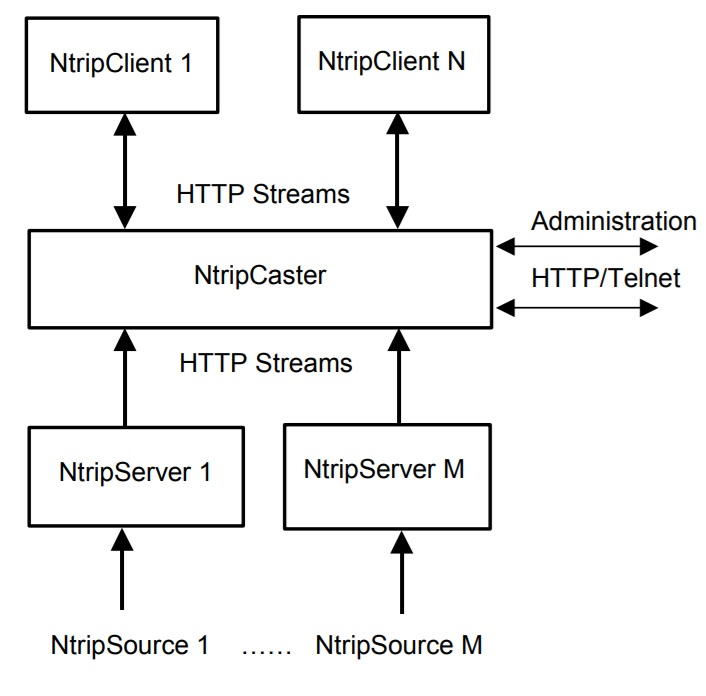
\includegraphics[scale=0.65]{NTRIP.jpg}
	\caption{NTRIP streaming systeem}
	\cite{LBibNTRIP}
	\label{imgNTRIP}
\end{figure} 
 




\chapter{Reeds gerealiseerde elementen}
Dit hoofdstuk handelt de reeds gerealiseerde elementen. \newline
Als eerste zijn de doelstelling en het situering uitgeschreven en besproken in hoofdstuk \ref{Situering}. \newline
Als tweede is er theoretisch onderzoek gedaan naar satellieten, GNSS, EPN, RINEX, RTCM en NTRIP. Dit onderzoek is verwerkt en is terug te vinden in hoofdstuk \ref{Literatuurstudie}. \newline
Voor de rest is er momenteel nog niet veel gebeurd. Dit doordat er pas laat met het onderwerp begonnen is en momenteel de contracten met de Koninklijke Sterrenwacht nog niet op punt staan. Hierdoor kan de student daar nog niet praktisch aan de slag. Er wordt gepland dat dit tegen begin januari in orde is en de student dan kan beginnen. Hoofdstuk \ref{Planning} beschrijft de verdere planning voor deze masterproef.

\chapter{Planning}
\label{Planning}
Dit hoofdstuk is het het laatste hoofdstuk van het tussentijds verslag. Het omschrijft de planning voor de komende maanden. 

Figuur \ref{imgGant} toon een grafische weergave van de planning in de vorm van een Gantt kaart. 

\begin{figure}[hpb]
	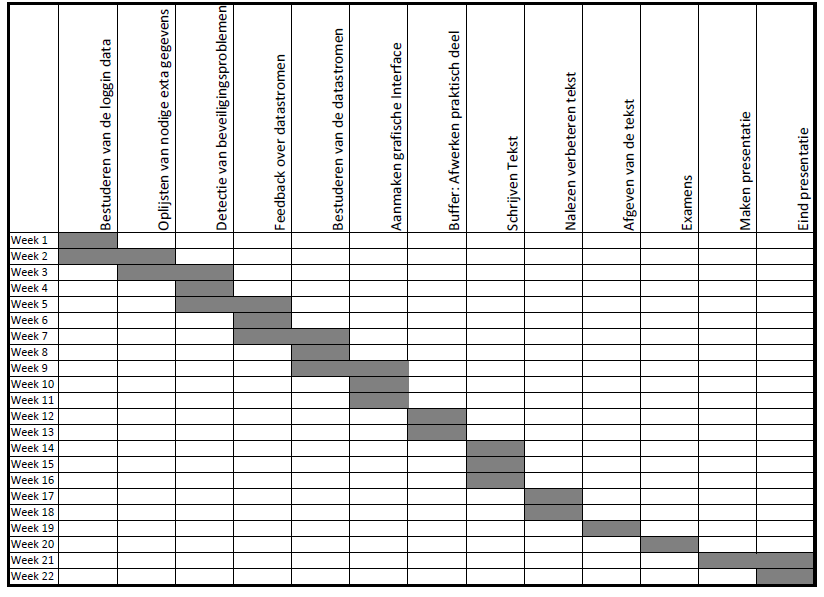
\includegraphics[scale=0.95]{Gantt.png}
	\caption{Gantt Shart}
	\label{imgGant}
\end{figure} 

Hierbij is week 1 de week van 15 tot en met 21 januari. Week 22 is de week van 24 juni. Naar schatting vallen daar ongeveer de masterproef verdedigingen. 
Er is een periode van drie weken voorzien om de tekst te schrijven. Natuurljk is dit niet voldoende. De tekst wordt tussendoor ook geschreven. Deze drie weken is voor het afronden van de tekst. 


% Bibliografie: referenties. De items zitten in bibliografie.bib
%%%%%%%%%%%%%%%%%%%%%%%%%%%%%%%%%%%%%%%%%%%%%%%%%%%%%%%%%%%%%%%%%
% Indien je ook de niet geciteerde werken in je bibliografie wil opnemen, commentarieer dan onderstaande regel uit!
%\nocite{*}
\bibliographystyle{ieeetr}
\bibliography{bibliografie}

% Eventueel enkele appendices
%%%%%%%%%%%%%%%%%%%%%%%%%%%%%%

% Bijlage met daarin het wetenschappelijk artikel
%%%%%%%%%%%%%%%%%%%%%%%%%%%%%%%%%%%%%%%%%%%%%%%%%%
%\includepdf{artikel.pdf}

% Bijlage met daarin de poster
%%%%%%%%%%%%%%%%%%%%%%%%%%%%%%%
%\includepdf{poster.pdf}


\includepdf{back_fiiw_denayer.pdf}
% 
\includepdf{back_fiiw_denayer_eng.pdf} % For the english version

\end{document}
